\documentclass[11pt,a4paper]{report}

\usepackage{polski}
\usepackage[utf8]{inputenc} 
\usepackage{a4wide}
\usepackage{tabularx}
\usepackage{lastpage}
\usepackage{fancyhdr}
\usepackage{graphicx}
\usepackage{caption}


% strona tytułowa
\begin{titlepage}
\title{\Huge Sprawozdanie z Projektu\\\textsl{Tanks}}
\author{Daniel Ślusarczyk i Jakub Łaba}
\date{09.06.2021}
\end {titlepage}

\renewcommand{\footrulewidth}{0pt}
\begin{document}
\maketitle

% zmiana numeracji sekcji 0.X -> X
\renewcommand*\thesection{\arabic{section}} 
\begin{abstract}
Dokument stanowi sprawozdanie z projektu \textsl{"Tanks"}, z wyszczególnionym opisem aktualnego stanu projektu, zmian względem specyfikacji oraz wnioskami.
\end{abstract}

% numeracja stron
\pagestyle{fancy}
\fancyhf{}
\rhead{\textsl{Sprawozdanie z projektu "Tanks" | D. Ślusarczyk, J. Łaba}}
\rfoot{Strona \thepage \hspace{1pt} z \pageref{LastPage}}
\setcounter{page}{0}

% spis treści bez numeracji stron
\fancypagestyle{plain}
{
\fancyhead{} 
\fancyfoot{} 
}
\thispagestyle{empty} 
\tableofcontents 
\thispagestyle{empty}
\newpage

\fancypagestyle{plain} 
{
\fancyhead{} 
\fancyfoot[C]{\thepage}
}


% pierwsza sekcja
\section{Zarys Projektu}\label{sec:tekst}
Projekt  \textsl{"Tanks"} zakładał stworzenie programu dedykowanego dwóm graczom rozmieszczonym po dwóch stronach okna rozgrywki, których zadaniem jest strzelanie do komórek w środkowej części okna za pomocą przypisanych czołgów. Gracze maja możliwość wertykalnego poruszania się swoimi jednostkami, oraz obracania lufą czołgu. Każdy pojazd strzela pociskami o cechach możliwych do określenie przez plik konfiguracyjny. \\
Kwadratowe komórki, które są obiektem przyznawania punktów graczom, dzielą się na trzy rodzaje:
\begin {itemize}
\item \textbf {Zwykła komórka} --  kwadratowy obiekt o wszystkich krawędziach wrażliwych na kontakt z pociskiem. Punkty za jej unicestwienie przyznawane są graczowi zadającemu końcowe obrażenia.
\item \textbf {Bomba} -- obiekt posiadający niewrażliwe krawędzie z pominięciem górnej, która jest jedynym sposobem na zastrzelenie tej komórki. Dokonanie tego kończy grę.
\item \textbf {Kolonia} -- zbiór maksymalnie pięciu zwykłych komórek w losowej konfiguracji. Gracz otrzymuje zsumowane punkty wszystkich komórek wchodzących w skład kolonii po zastrzeleniu ostatniej komórki w zbiorze.
\end {itemize}
Wszystkie wyżej wymienione komórki poruszają wertykalnie w dół w ramach okna rozgrywki. Podobnie jak pociski posiadają parametry modyfikowalne z poziomu pliku konfiguracyjnego, a ich najważniejszą cechą jest wartość potrzebna do zastrzelenia znajdująca się w centralnej części komórki.\\
Gra w sposób regularny zwiększa trudność rozgrywki poprzez zwiększanie wartości potrzebnej do unicestwienia komórki, szybkości komórek i wystrzeliwanych pocisków, oraz zmniejszanie promienia pocisku i długości boku komórki. Koniec gry przewidują dwa scenariusze: upłyniecie określonego czasu rozgrywki lub zastrzelenie komórki bomby. Grę wygrywa gracz o większej ilości punktów w momencie zakończenia.
\newpage
% druga sekcja
\section{Struktura programu}\label{sec:tekst}
\subsection {Struktura katalogów}
Folder \textsl{tanks} jest głównym folderem projektowym, w ramach którego mieszczą się wszystkie pliki związane z projektem. Zawiera dwa foldery i jeden plik: 
\begin{itemize}
\item{Dokumenty}\\
Folder \textsl{dokumenty} przechowuje specyfikację funkcjonalną i implementacyjną, oraz sprawozdanie końcowe. Każdy z tych dokumentów znajduje się w osobnych folderze, który zawiera pliki związane wyłącznie z danym dokumentem.
\item{Src}\\
Folder \textsl{src} jest katalogiem związanym z kodem i działaniem przygotowanego oprogramowania. W podkatalogu o ścieżce \textsl{test/java} przechowuje przygotowane testy automatyczne oprogramowania. Natomiast w podkatalogu \textsl{main} przechowywany jest kod źródłowy projektu, folder do zapisu wykonanych zrzutów ekranu i pliki niezbędne do działania programu, a w szczególności pliki konfiguracyjne. 
\item{Pom.xml}\\
Plik zawierający informacje o projekcie i szczegóły używane przez narzędzie automatyzujące budowę oprogramowania \textsl{Maven}.

\end{itemize}
\newpage
\begin{figure}[!ht]
\centerline{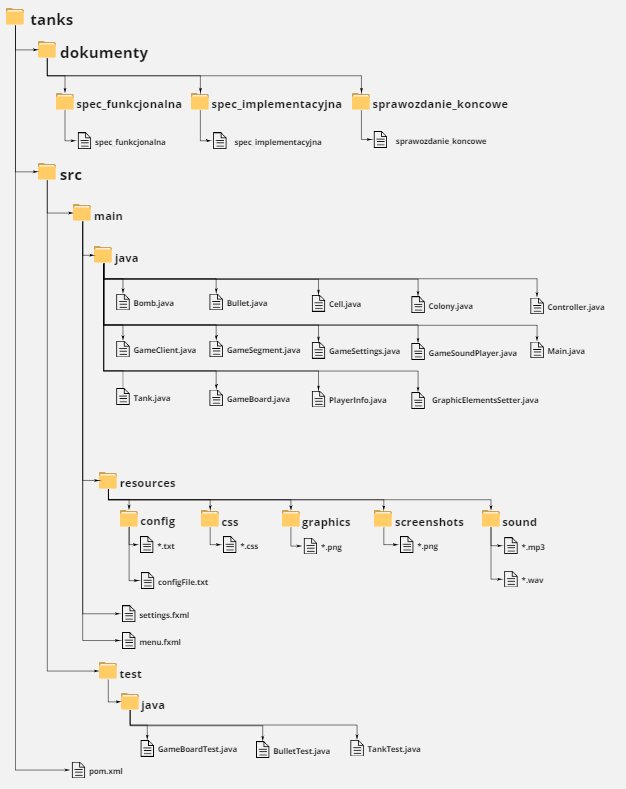
\includegraphics{img/struktura.png}}
\caption{Schemat struktury katalogów}
\end{figure}
\newpage

% trzecia sekcja
\section{Szczegóły oprogramowania}
\subsection {Narzędzie automatyzujące budowę "Maven"}
Do stworzenia gry został wykorzystany \textsl{Maven} -- jest to narzędzie upraszczające pracę nad tworzeniem aplikacji, zwłaszcza korzystających z dużej ilości modułów -- co w przypadku mocno podzielonego na moduły frameworku graficznego \textsl{JavaFX} jest pomocne. Najważniejsze moduły załączone w aplikacji za pomocą \textsl{Maven}-a to:
\begin{itemize}
\item \textbf {JavaFX Graphics}
\item \textbf {JavaFX Controls}
\item \textbf {JavaFX FXML}
\item \textbf {JavaFX Media}
\item \textbf {JUnit5}
\end{itemize}
\subsection {Automatyczne testy}
Aplikacja została przetestowana za pomocą testów jednostkowych z wykorzystaniem biblioteki \textsl{JUnit} w wersji \texttt{5.7.0}. Przetestowane zostały metody odpowiadające za poruszanie oraz usuwanie poszczególnych komponentów rozgrywki.
\subsection {Zasady działania elementów}
\subsubsection{Kolonie}
Generowanie kolonii odbywa się na podstawie kwadratu o wymiarach 3x3 komórki. Środkowe pole kwadratu jest zawsze zajmowane przez komórkę, a dodatkowo jest losowane od 1 do 4 komórek, które zajmują losowe miejsca dookoła niej. Wszystkie komórki zmniejszają się o wartość DH1 co T1 sekund. Unicestwienie kolonii wymaga unicestwienia wszystkich komórek należących do zbioru. Komórki, które zostały trafione wystarczającą ilość razy i należą do kolonii są wyświetlane z cyfrą 0 i stają się niewrażliwie na pociski. Trafienie ostatniej komórki powoduje zniknięcie wszystkich elementów kolonii i naliczenie punktów graczowi, który tego dokonał.
\subsubsection{Pociski}
\textsl{Bullet} jest klasą dziedziczącą po \textsl{GameSegment} -- został on rozszerzony o dane dotyczące wektora, opisującego tor ruchu danego pocisku. Wektor jest obliczany już w konstruktorze, który jest wywoływany w metodzie \textsl{shoot()} klasy \textsl{Tank} -- pocisk powstaje w momencie jego wystrzelenia. Poniższy schemat wizualizuje kilka istotnych zależności, wykorzystanych w celu odpowiedniego umieszczania i poruszania się pocisków.
\begin{figure}[!ht]
\centerline{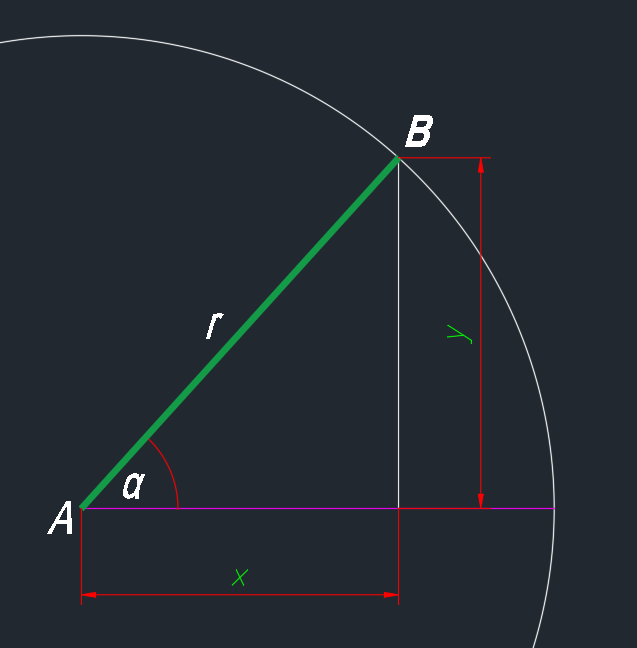
\includegraphics{img/schemat_lufa.png}}
\caption{Schemat przedstawiający lufę czołgu (zaznaczona kolorem zielonym)}
\end{figure}
Punkt A jest jest współrzędnymi czołgu przechowywanymi w polach klasy \textsl{Tank}, natomiast punkt B reprezentuje czubek lufy -- miejsce w którym w momencie wystrzału powinien pojawić się pocisk. Długość lufy jest reprezentowana przez r, ta wartośc również jest przechowywana jako pole w klasie \textsl{Tank}. Wektorem ruchu pocisku jest wektor $\vec{AB}$.\\\\
Przyjmując \[A = (x_a, y_a)\]\[B = (x_b, y_b)\]
Otrzymujemy \[x = x_b - x_a\]\[y = y_a - y_b\] \[\vec{AB} = [x_b - x_a, y_b - y_a] = [x, -y]\]
Wówczas \[sin\alpha= \frac{y_a - y_b}{r}\] \[cos\alpha = \frac{x_b - x_a}{r}\]
Zatem \[x = rcos\alpha\]\[y = rsin\alpha\]\[\vec{AB} = [rcos\alpha, -rsin\alpha]\]\[B = (x_a + x, y_a - y)\]
\subsection {Licencje elementów}
Przygotowane oprogramowanie korzysta z plików graficznych i dźwiękowych udostępnionych przez autorów na zasadach licencji pozwalających na legalne wykorzystanie ich w projekcie \textsl{"Tanks"}.
\subsubsection{Informacje o poszczególnych elementach:}
\begin {itemize}
\item{Wszystkie elementy graficzne:}\\
Źródło: \textsl{https://opengameart.org/content/tank-2}\\
Autor: KASTLE Knight\\
Licencja: CC 1.0
\item{Muzyka w tle: }\\
Źródło: \textsl{https://freesound.org/people/bipwave/sounds/505985/}\\
Autor: bipwave\\
Licencja: CC 1.0
\item{Muzyka końca gry:}\\
Źródło: \textsl{https://freesound.org/people/kimp10/sounds/341578/}\\
Autor: kimp10\\
Licencja: CC 1.0
\item{Efekty dźwiękowe:}\\
Źródło: \textsl{https://mixkit.co/free-sound-effects/music/}\\
Licencja: Mixkit Sound Effects Free License
\end {itemize}
\newpage

% czwarta sekcja
\section{Przegląd programu}\label{sec:teskt}
Przedstawione poniżej elementy prezentują różne funkcjonalności oprogramowania.
\subsection {Elementy obsługi gry}
\subsubsection{Okno menu}
Poniższy rysunek przedstawia okno menu widziane jako pierwszy element po uruchomieniu oprogramowania.
\begin{figure}[!ht]
\centerline{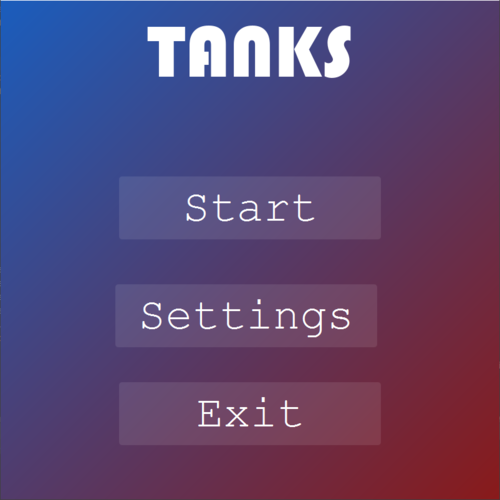
\includegraphics{img/menu.png}}
\caption{Okno menu }
\end{figure}
\newpage
\subsubsection{Okno ustawień}
\begin{itemize}
\item{Pierwsza zakładka}\\
Z poziomu pierwszej zakładki użytkownik ma możliwość ustawienia niektórych elementów działania program --  dostosowanie głośności dźwięku, wczytanie własnego pliku konfiguracyjnego i zaznaczenie wykonywania zdjęcia po zakończonej rozgrywce. 
\begin{figure}[!ht]
\centerline{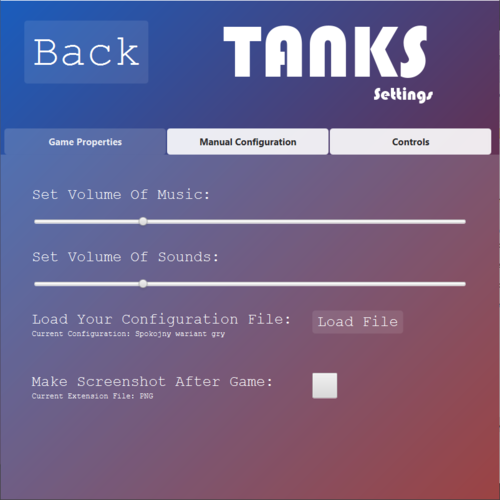
\includegraphics{img/zakladka1.png}}
\caption{Zakładka Game Properties }
\end{figure}
\newpage
\item{Druga zakładka}\\
Z poziomu drugiej zakładki użytkownik ma możliwość dostosowania poszczególnych elementów pliku konfiguracyjnego. Dodatkowo na samym dole znajduje się przycisk, który po podaniu żądanej nazwy pliku jest w stanie stworzyć plik konfiguracyjny o podanej nazwie w formacie zgodnym z oprogramowaniem i zapisać zmiany.
\begin{figure}[!ht]
\centerline{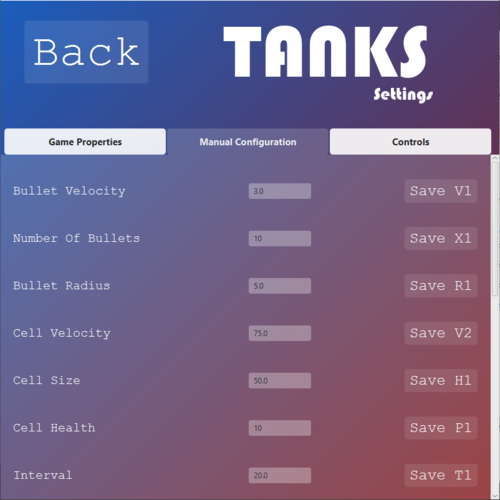
\includegraphics{img/zakladka2.png}}
\caption{Zakładka Manual Configuration }
\end{figure}
\newpage
Podanie wartości o niezgodnym formacie i próba zapisu do pliku powoduje podświetlenie niewłaściwych pól na czerwono i zaakceptowanie tylko tych prawidłowych.
\begin{figure}[!ht]
\centerline{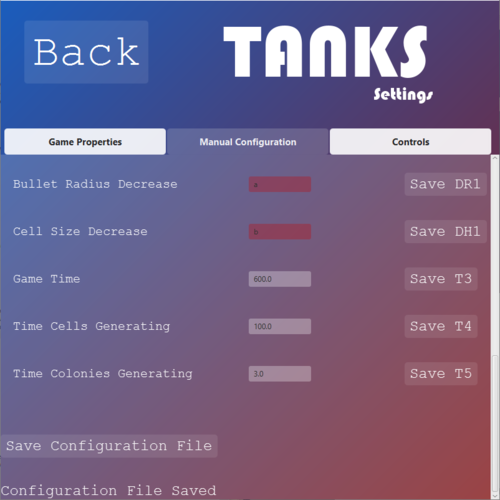
\includegraphics{img/zakladka2.1.png}}
\caption{Zakładka Manual Configuration }
\end{figure}
\newpage
\item{Trzecia zakładka}\\
Z poziomu trzeciej zakładki użytkownik ma możliwośc przypisania w sposób dowolny sterowania gry dla obu użytkowników.
\begin{figure}[!ht]
\centerline{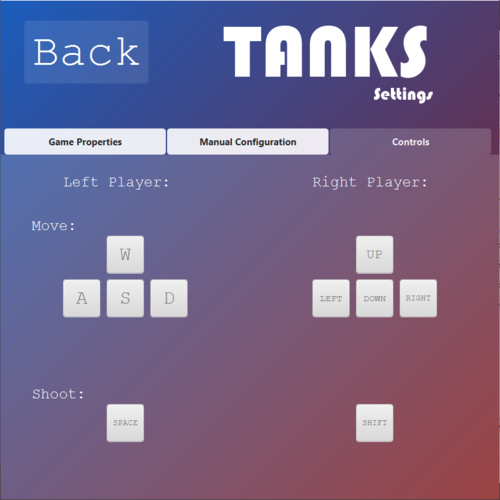
\includegraphics{img/zakladka3.png}}
\caption{Zakładka Manual Configuration }
\end{figure}
\newpage
Próba przypisania sterowania do wykorzystywanego przycisku powoduje podświetlnie na czerwono miejsca, w którym jest przypisany i niezapisanie zmian.
\begin{figure}[!ht]
\centerline{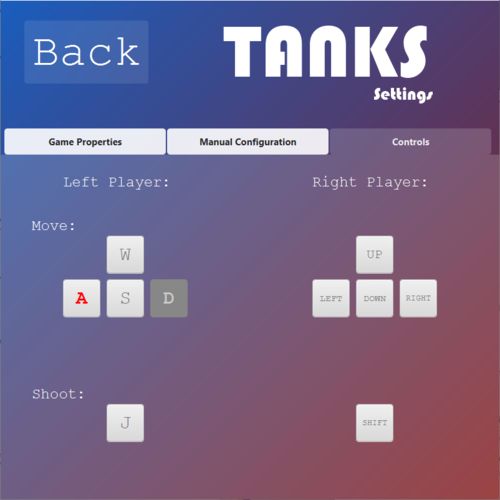
\includegraphics{img/zakladka3.1.png}}
\caption{Zakładka Manual Configuration }
\end{figure}
\newpage
\subsubsection{Elementy Statyczne Rozgrywki}
\item{Koniec gry}\\
Zakończenie rozgrywki prezentowane jest przez poniższe okno. Udostępnia ono informacje w formie diagramu kołowego o ilości punktów uzyskanych przez poszczególnych graczy i daje możliwość wyjścia z gry, lub ponownego uruchomienia rozgrywki. Jeśli w ustawieniach zostało zaznaczone miejsce ustawiające wykonanie zrzutu ekranu to w folderze \textsl{'resources/screenshots'} zostanie zapisy zrzut ekranu tego okna.
\begin{figure}[!ht]
\centerline{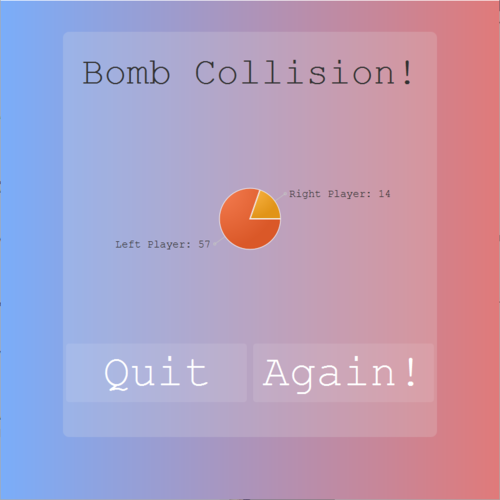
\includegraphics{img/koniec.png}}
\caption{ Okno końca gry }
\end{figure}
\newpage
\item{Wstrzymanie gry}\\
Naciśnięcie przycisku "P" powoduje zatrzymanie działania gry i oczekiwanie na dalsze czynności użytkownika. Z poziomu wyświetlanego okna można wznowić grę, lub przejść do okna ustawień.
\begin{figure}[!ht]
\centerline{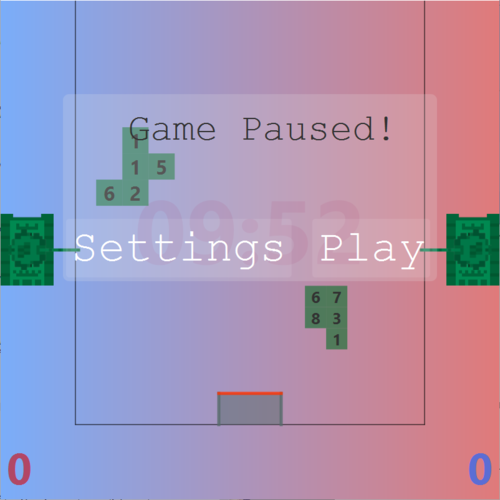
\includegraphics{img/stop.png}}
\caption{ Okno Wstrzymania Gry }
\end{figure}
\end{itemize}
\newpage


\subsection {Rozgrywka}
\begin{itemize}
\item{}Okno wyświetlane podczas stanardowej rozgrywki zawiera takie elementy jak: punktacje obu graczy, czołgi obu graczy, czas do końca rozgrywki, komórki,  kolonie i miejsce wyświetlania komunikatów o ewentualnych błędach.
\begin{figure}[!ht]
\centerline{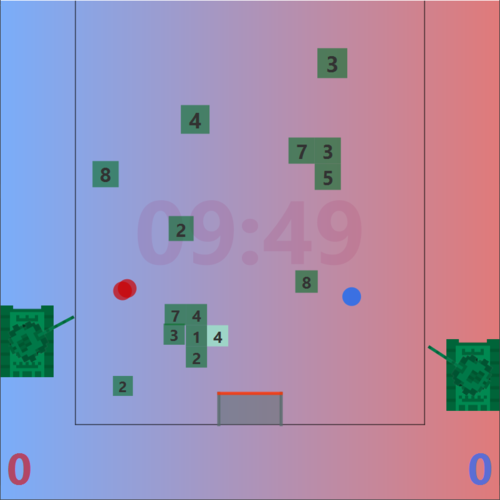
\includegraphics{img/rozgrywka1.png}}
\caption{ Przykład rozgrywki }
\end{figure}
\newpage
\item{}Kolonia z ostatnią żywą komórką wyświetlana jest w następujący sposób.
\begin{figure}[!ht]
\centerline{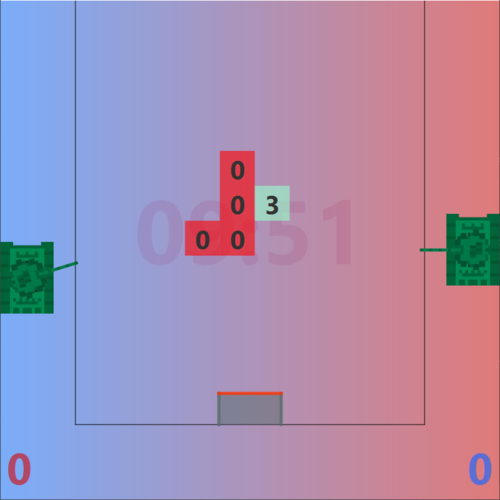
\includegraphics{img/rozgrywka2.png}}
\caption{ Przykład rozgrywki }
\end{figure}
\newpage
\item{}Kololonia wyświetlana dla wartości H1 równej 120.
\begin{figure}[!ht]
\centerline{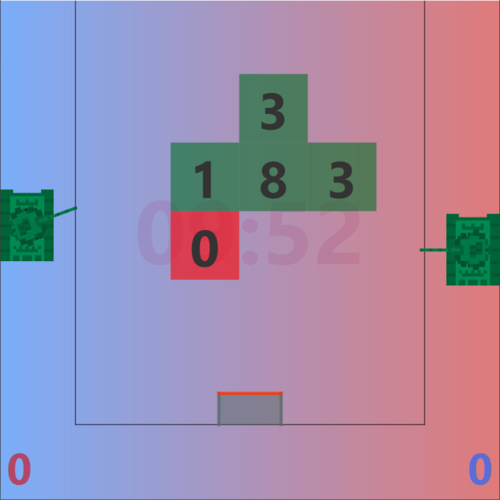
\includegraphics{img/rozgrywka3.png}}
\caption{ Przykład rozgrywki }
\end{figure}
\newpage
\item{}Pociski gracza dla wartości X1 równej 1000 i V1 równej 8.
\begin{figure}[!ht]
\centerline{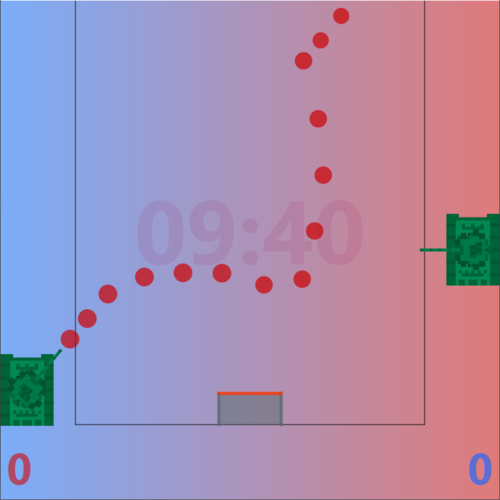
\includegraphics{img/rozgrywka4.png}}
\caption{ Przykład rozgrywki }
\end{figure}
\newpage
\item{}Pojedyncze komórki dla wartości H1 równej 120, DH1 równej 20 i V2 równej 100.
\begin{figure}[!ht]
\centerline{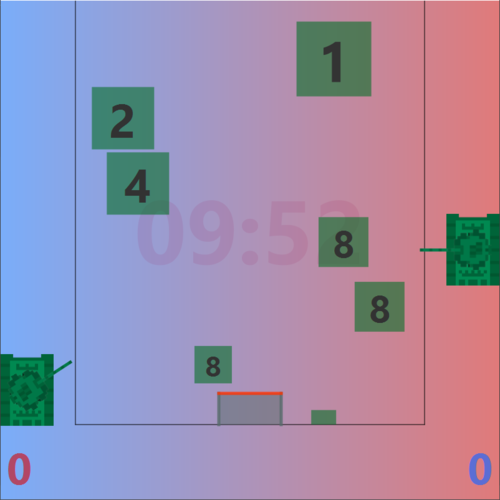
\includegraphics{img/rozgrywka5.png}}
\caption{ Przykład rozgrywki }
\end{figure}
\newpage
\item{}Okno rozgrywki z komunikatami o naciśnięciu przycisków, które nie są przypisane do żadnego sterowania.
\begin{figure}[!ht]
\centerline{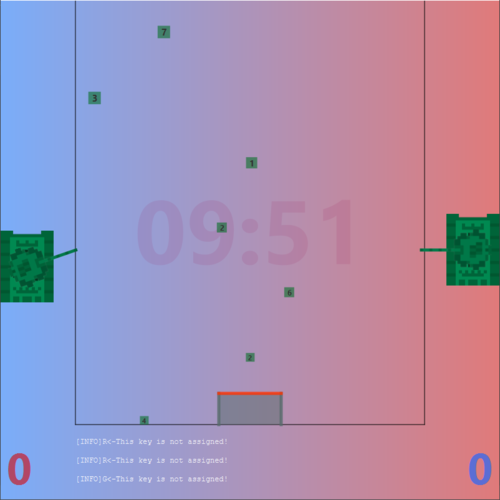
\includegraphics{img/rozgrywka6.png}}
\caption{ Przykład rozgrywki }
\end{figure}
\end{itemize}
\newpage


% piąta sekcja
\section{Zmiany względem specyfikacji}\label{sec:teskt}
Założeniem projektu od samego początku powstawania było zachowanie ścisłości między pisanym programem, a specyfikacją funkcjonalna i implementacyjną. Proces powstawania elementów projektu zweryfikował dokładnie wszystkie założone idee i spowodował zmianę niektórych elementów.
\subsection {Plik konfiguracyjny}
Plik konfiguracyjny został wzbogacony o dwie dodatkowe zmienne:
\begin{itemize}
\item{}[T4] TimeBetweenCellGenerating [liczba rzeczywista] -- pozwala określić czas pomiędzy kolejnymi wygenerowanymi komórkami.
\item{}[T5] TimeBetweenColonyGeneration [liczba rzeczywista] -- pozwala określić czas pomiędzy kolejnymi wygenerowanymi koloniami.
\end{itemize}
\subsection {Funkcjonalności programu}
W funkcjonalnościach programu zrezygnowano z trzech predefiniowanych trybów trudności. Niemniej jednak, zostało dododane znacznie bardziej rozbudowane okno ustawień. Dodatkowo okno błędów ma możliwość nie tylko informowania o ewentualnych błędach, ale również np. o naciśnietych przyciskach, które nie są nigdzie przypisane.
 
\subsection {Aktualny uproszczony diagram klas}
W trakcie prac nad projektem, zostały utworzone dwie  nowe klasy -- \textsl{GraphicElementsSetter} oraz \textsl{GameSoundPlayer}.
\textsl{GraphicElementsSetter} jest odpowiedzialny za tworzenie graficznych komponentów gry -- klasa ta powstała w celu zredukowania ilości metod w klasie \textsl{Controller}.
Dodanie do gry dźwięku wymusiło stworzenie  klasy \textsl{GameSoundPlayer}, obsługującej metody związane z odtwarzaniem go.
\newpage
\begin{figure}[ht!]
\centerline{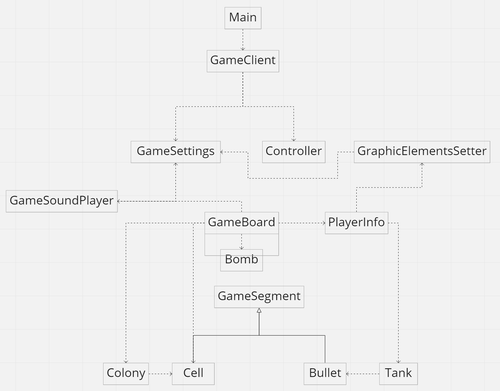
\includegraphics{img/diagram_klas.png}}
\caption{Uproszczony diagram UML, pokazujący zależności pomiędzy klasami}
\end{figure}

\newpage

% szósta sekcja
\section{Podsumowanie współpracy}\label{sec:teskt}
Współpraca w obrębie projektu \textsl{Tanks} przebiegała bez zauważalnych problemów. Głównymi czynnikiami wyraźnie ułatwiającymi współpracę było korzystanie z podobnych narzędzi programistycznych i doświadczenie wyniesione z poprzednich projektów.
\subsection {Systematyczność}
Równolegle z uczelnianym repozytorium \textsl{Projektor} korzystaliśmy również z \textsl{Githuba} głównie z powodu możliwości dodania wielu kluczy \texttt{SSH} dla pojedynczego użytkownika -- istotność potrzeby takiej funkcjonalności wynika z faktu, że obu autorów kodu pracowało na wielu urządzeniach bądź maszynach wirtualnych.\\ Dane dotyczące repozytorium \texttt{https://github.com/jakublaba/tanks} na dzień \texttt{9.06.2021}:\\
\begin{figure}[ht!]
\centerline{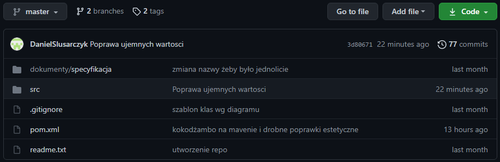
\includegraphics{img/repo.png}}
\caption{Strona główna repozytorium, ukazująca ilość commit-ów}
\end{figure}
\newpage
\begin{figure}[ht!]
\centerline{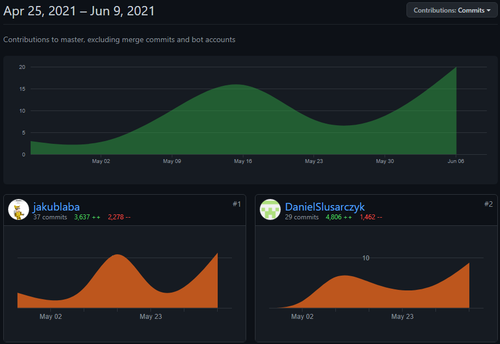
\includegraphics{img/contributors.png}}
\caption{Wykresy ukazujące częstotliwośc commit-ów poszczególnych użytkowników repozytorium}
\end{figure}
\newpage
\begin{figure}[ht!]
\centerline{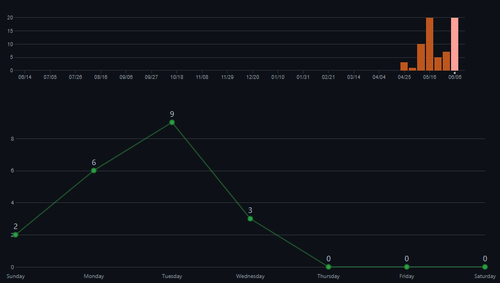
\includegraphics{img/commits.png}}
\caption{Wykresy ukazujące ogólną częstotliwość commit-ów}
\end{figure}
\begin{figure}[ht!]
\centerline{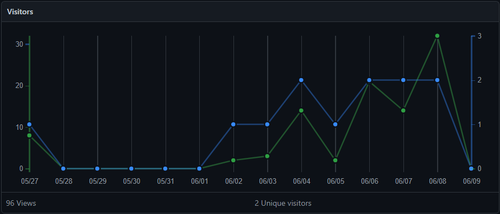
\includegraphics{img/visitors.png}}
\caption{Wykres ukazujący częstotliwość odwiedzania repozytorium}
\end{figure}
\newpage
\begin{figure}[ht!]
\centerline{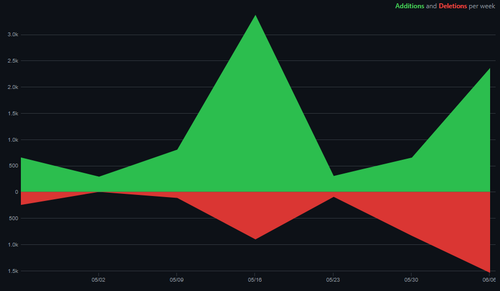
\includegraphics{img/code_frequency.png}}
\caption{Wykres ukazujący średnie tygodniowe ilości edytowanych linii kodu}
\end{figure}

\newpage

% siódma sekcja
\section{Podsumowanie projektu}\label{sec:teskt}
Projekt  \textsl{"Tanks"} został w całości przygotowany od 15.04.2021 do 09.06.2021. W ramach niego powstała działająca gra dedykowana dwóm graczom, specyfikacja implementacyjna, specyfikacja funkcjonalna oraz sprawozdanie końcowe. Przygotowane rozwiązanie korzysta zarówno z elementów graficznych, jak również wielu narzędzi programistycznych dostarczanych przez język programowania obiektowego „Java”. Poprzez modyfikowalny plik konfiguracyjny każdy odbiorca oprogramowania ma możliwość w prosty sposób dostosować wiele elementów rozgrywki zgodnie z własnymi upodobaniami, a dzięki intuicyjnemu interfejsowi aplikacji obsługa programu jest bardzo prosta nawet dla niezaawansowanych użytkowników. Całe oprogramowanie było tworzone w oparciu o narzędzie automatyzujące budowę „Maven”, które pozwala w sposób uporządkowany zarządzać działaniem programu przez różne osoby mające styczność z kodem źródłowym programu.


% ósma sekcja
\section{Wnioski}\label{sec:teskt}
 Projekt  \textsl{"Tanks"} był zadaniem, który pozwolił na dostrzeżenie esencji programowania obiektowego w języku „Java”. Konieczność zdefiniowana w tym projekcie obiektów abstrakcyjnych, które łączą wspólne zależności i wzajemnie ze sobą współgrają umożliwiło zgłębienie koncepcji stojącej za programowaniem obiektowym i zrozumieć działanie mechanizmów z nim związanych. Dodatkowo konieczność stworzenia interfejsu graficznego unaoczniła trudności związane z tworzeniem warstwy graficznej i połączeniem jej z logicznym działaniem oprogramowania.


\end{document}